\section{Проект}
\label{sec:project}

В данном разделе описываются принятые при разработке проектные решения, внутренняя структура программной системы, используемые средства реализации и стандарты кодирования.

\subsection{Средства реализации}

При разработке системы проводился сравнительный анализ инструментов и технологий для выбора оптимального стека.

\subsubsection*{Язык программирования}

В качестве основного языка программирования выбран \textbf{Python 3.11+}.

\textbf{Обоснование выбора:}
\begin{itemize}
    \item \textbf{Библиотеки компьютерного зрения}: Python обладает наиболее полной экосистемой библиотек для работы с изображениями и нейронными сетями (OpenCV, PyTorch, EasyOCR), что является критическим требованием для данной системы.
    \item \textbf{Скорость разработки}: динамическая типизация и высокий уровень абстракции позволяют быстро прототипировать и тестировать алгоритмы, что особенно важно для учебной разработки.
    \item \textbf{Кроссплатформенность}: код может выполняться на Windows, Linux и macOS без существенных изменений.
    \item \textbf{Интеграция с Windows API}: библиотека \texttt{pywin32} предоставляет удобный доступ к функциям захвата окон, необходимых для работы с покер-клиентом.
\end{itemize}

\textbf{Альтернативы:}
\begin{itemize}
    \item \textbf{C++}: обеспечил бы более высокую производительность, но значительно усложнил бы разработку и интеграцию с нейросетевыми библиотеками.
    \item \textbf{C\#}: хорошая интеграция с Windows, но менее развитая экосистема библиотек компьютерного зрения.
\end{itemize}

\subsubsection*{Библиотеки компьютерного зрения и OCR}

\begin{itemize}
    \item \textbf{OpenCV 4.x} --- основная библиотека для обработки изображений (предобработка, морфологические операции, работа с цветовыми пространствами HSV/RGB). Выбрана как отраслевой стандарт с открытым исходным кодом.
    
    \item \textbf{EasyOCR} --- библиотека оптического распознавания текста на базе PyTorch. Выбрана вместо Tesseract по следующим причинам:
    \begin{itemize}
        \item лучшая точность распознавания текста на игровых интерфейсах с нестандартными шрифтами;
        \item встроенная поддержка GPU для ускорения обработки;
        \item простота интеграции и настройки.
    \end{itemize}
    
    \item \textbf{YOLOv8 + ResNet18} (в модуле \texttt{CardExtractor}) --- используются для детекции и классификации карт. YOLOv8 обеспечивает быструю детекцию объектов, ResNet18 --- точную классификацию рангов и мастей.
\end{itemize}

\subsubsection*{Графический интерфейс}

\begin{itemize}
    \item \textbf{PyQt6} --- фреймворк для создания оверлейного окна. Выбран благодаря:
    \begin{itemize}
        \item возможности создания прозрачных окон с атрибутом;
        \item поддержке режима \texttt{click-through}, что позволяет не блокировать взаимодействие с покер-клиентом;
        \item функции для отображения поверх всех окон.
    \end{itemize}
\end{itemize}

\subsubsection*{Системные библиотеки}

\begin{itemize}
    \item \textbf{pywin32} --- предоставляет доступ к Windows API для захвата изображений окон через функции \texttt{PrintWindow} и \texttt{GetWindowDC}.
    \item \textbf{NumPy} --- эффективная работа с многомерными массивами (изображения представляются как матрицы пикселей).
    \item \textbf{logging} --- стандартный модуль Python для логирования, обеспечивает гибкую настройку уровней детализации.
\end{itemize}

\subsubsection*{Среда разработки}

Разработка велась в среде \textbf{Visual Studio Code} с использованием расширений:
\begin{itemize}
    \item Python (Microsoft) --- интеллектуальное завершение кода, линтинг;
    \item Pylance --- статический анализ типов;
\end{itemize}

Для управления зависимостями использовался \textbf{pip} с виртуальным окружением \texttt{venv}.

\subsection{Структуры данных}

В системе используются следующие основные структуры данных.

\subsubsection*{Доменные сущности}

\textbf{Card} --- представляет игральную карту:
\begin{itemize}
    \item \texttt{rank: str} --- ранг карты (2--10, J, Q, K, A);
    \item \texttt{suit: str} --- масть (hearts, diamonds, clubs, spades).
\end{itemize}

\textbf{Player} --- информация об игроке:
\begin{itemize}
    \item \texttt{seat: int} --- номер места за столом (0--5);
    \item \texttt{nickname: str} --- имя игрока;
    \item \texttt{stack: float} --- размер стека в фишках;
    \item \texttt{position: str} --- позиция (UTG, MP, CO, BTN, SB, BB);
    \item \texttt{is\_hero: bool} --- флаг, является ли игрок героем (пользователем);
    \item \texttt{is\_button: bool} --- флаг наличия кнопки дилера;
    \item \texttt{is\_active: bool} --- участвует ли в текущей раздаче;
    \item \texttt{cards: List[Card]} --- карты игрока;
    \item \texttt{last\_bet: float} --- последняя сделанная ставка;
    \item \texttt{zone: Optional[Rect]} --- область на экране, занимаемая игроком;
    \item \texttt{last\_ocr\_time: float} --- время последнего распознавания текста.
\end{itemize}

\textbf{PokerTable} --- состояние игрового стола:
\begin{itemize}
    \item \texttt{players: List[Player]} --- список игроков;
    \item \texttt{community\_cards: List[Card]} --- общие карты на столе;
    \item \texttt{is\_hero\_turn: bool} --- флаг очереди хода героя;
    \item \texttt{small\_blind, big\_blind: float} --- размеры блайндов;
    \item \texttt{preflop\_action: PreflopActionInfo} --- информация о префлоп-действиях;
    \item \texttt{pot: float} --- размер банка;
    \item \texttt{street: str} --- улица торговли (preflop, flop, turn, river).
\end{itemize}

\textbf{PreflopActionInfo} --- детализация префлоп-ситуации:
\begin{itemize}
    \item \texttt{is\_open\_raise: bool} --- является ли ситуация открытием торговли;
    \item \texttt{is\_3bet\_pot, is\_4bet\_pot: bool} --- был ли 3-бет/4-бет;
    \item \texttt{first\_raiser\_seat, first\_raiser\_position} --- кто открылся первым;
    \item \texttt{three\_bettor\_seat, three\_bettor\_position} --- кто сделал 3-бет;
    \item \texttt{callers: List[int]} --- список игроков, сделавших колл;
    \item \texttt{hero\_to\_call\_bb: float} --- сколько герою нужно уравнять в больших блайндах.
\end{itemize}

\subsubsection*{Геометрические структуры}

\textbf{Rect} (прямоугольник):
\begin{itemize}
    \item \texttt{x1, y1: int} --- координаты левого верхнего угла;
    \item \texttt{x2, y2: int} --- координаты правого нижнего угла;
    \item \texttt{width, height} (вычисляемые свойства) --- размеры прямоугольника.
\end{itemize}

\textbf{Point} (точка):
\begin{itemize}
    \item \texttt{x, y: int} --- координаты точки.
\end{itemize}

\subsubsection*{Структуры для рекомендаций}

\textbf{Advice} --- рекомендация для игрока:
\begin{itemize}
    \item \texttt{action: ActionRecommendation} --- рекомендуемое действие (FOLD, CALL, RAISE);
    \item \texttt{confidence: Confidence} --- уровень уверенности (LOW, MEDIUM, HIGH);
    \item \texttt{reason: str} --- текстовое обоснование;
    \item \texttt{hand\_strength: Optional[float]} --- сила руки (0.0--1.0);
    \item \texttt{range\_coverage: Optional[float]} --- процент покрытия диапазона.
\end{itemize}

\textbf{Обоснование выбора структур:}
\begin{itemize}
    \item Использование \textbf{dataclasses} из стандартной библиотеки Python обеспечивает лаконичный синтаксис, автоматическую генерацию конструкторов и методов представления, что упрощает поддержку кода.
    \item \textbf{Optional} типы из модуля \texttt{typing} явно указывают на возможность отсутствия значения, что снижает риск ошибок \texttt{NoneType}.
    \item \textbf{Enum} для действий и уверенности обеспечивает типобезопасность и предотвращает использование недопустимых строковых значений.
\end{itemize}

\subsection{Модули и алгоритмы}

\subsubsection*{Общая архитектура системы}

Система построена по модульному принципу с чётким разделением ответственности.

\subsubsection*{Основные модули}

\textbf{1. Точка входа (\texttt{service.py})}

Основной цикл программы:
\begin{itemize}
    \item поиск окна покер-рума через \texttt{win32gui.EnumWindows};
    \item инициализация \texttt{PokerStateManager};
    \item бесконечный цикл захвата кадров и обновления состояния;
\end{itemize}

\textbf{2. Оркестратор (\texttt{PokerStateManager})}

Координирует работу всех подсистем:
\begin{itemize}
    \item делегирует обработку кадра объекту \texttt{Room};
    \item управляет обновлением оверлейного интерфейса;
    \item контролирует периодическое обновление блайндов (каждые 5 секунд);
    \item инициирует префлоп-анализ при наступлении очереди героя.
\end{itemize}

\textbf{3. Абстракция рума (\texttt{BaseRoom}, \texttt{ReplayPokerRoom})}

Инкапсулирует всю room-specific логику:
\begin{itemize}
    \item вычисление зон (игроки, ставки, общие карты);
    \item экстракция данных (карты, никнеймы, ставки);
    \item детекция очереди героя;
    \item определение позиций через \texttt{PositionAssigner}.
\end{itemize}

\textbf{4. Конвейер компьютерного зрения (\texttt{PokerVisionPipeline})}

Отвечает за геометрические вычисления:
\begin{itemize}
    \item определение центра стола;
    \item вычисление зоны общих карт (45\% ширины стола, 15\% высоты);
    \item определение зон игроков на основе пропорций (6 позиций с заданными коэффициентами);
    \item уточнение зон ставок через поиск тёмных панелей.
\end{itemize}

\textbf{5. Экстракторы}

\begin{itemize}
    \item \texttt{CardExtractor} --- использует YOLOv8 для детекции карт и ResNet18 для классификации;
    \item \texttt{BetExtractor} --- распознаёт суммы ставок через EasyOCR с предварительной обработкой (upscale 3x, бинаризация Otsu);
    \item \texttt{NicknameExtractor} --- извлекает имена игроков;
    \item \texttt{PlayerExtractor} --- агрегирует данные об игроках.
\end{itemize}

\textbf{6. Детекторы}

\begin{itemize}
    \item \texttt{HeroTurnDetector} --- определяет очередь героя через:
    \begin{itemize}
        \item поиск красных кнопок действий (HSV-маска красного цвета);
        \item распознавание текста кнопок (FOLD, CALL, RAISE);
        \item стабилизацию состояния (2 кадра подряд для избежания ложных срабатываний).
    \end{itemize}
    \item \texttt{DealerButtonDetector} --- находит кнопку дилера через template matching (\texttt{cv2.matchTemplate} с порогом 0.75).
\end{itemize}

\textbf{7. Модуль рекомендаций (\texttt{PreflopAdvisor})}

Реализует логику принятия решений:
\begin{itemize}
    \item классификация ситуации (RFI, VS\_OPEN, 3BET\_POT) на основе количества рейзов;
    \item парсинг диапазонов из формата Flopzilla (\texttt{RangeParser});
    \item сопоставление текущей руки с диапазоном (\texttt{hand\_matches\_range});
    \item формирование рекомендации с уровнем уверенности.
\end{itemize}

\textbf{8. Оверлейный интерфейс (\texttt{OverlayWindow}, \texttt{OverlayController})}

\begin{itemize}
    \item прозрачное PyQt6 окно с атрибутом \texttt{click-through};
    \item текстовое отображение состояния (карты, позиция, рекомендация);
    \item обновление в реальном времени через callback-механизм;
    \item цветовое кодирование действий (зелёный --- RAISE, красный --- FOLD, жёлтый --- CALL).
\end{itemize}

\subsubsection*{Ключевые алгоритмы}

\textbf{Алгоритм 1: Детекция очереди героя}

\begin{enumerate}
    \item Выделить область кнопок (60--100\% ширины, 65--98\% высоты экрана);
    \item Преобразовать в HSV цветовое пространство;
    \item Создать маску красного цвета (два диапазона: 0--10° и 160--180°);
    \item Применить морфологические операции (CLOSE, DILATE) для устранения шума;
    \item Подсчитать количество красных пикселей;
    \item Параллельно распознать текст кнопок через OCR;
    \item Если (красных пикселей > 10000) \textbf{И} (найдены keywords FOLD/CALL/RAISE) $\rightarrow$ очередь героя;
    \item Требовать стабильность 2 кадра подряд для подтверждения.
\end{enumerate}

\textbf{Алгоритм 2: Парсинг диапазонов}

Вход: строка в формате Flopzilla, например \texttt{"AA-55,AKs-A2s,KQo-K9o"}

\begin{enumerate}
    \item Разбить строку по запятым на токены;
    \item Для каждого токена:
    \begin{itemize}
        \item если диапазон пар (\texttt{55-22}) $\rightarrow$ сгенерировать все пары от старшей к младшей;
        \item если suited Ace range (\texttt{AKs-A2s}) $\rightarrow$ сгенерировать все Ax suited;
        \item если suited broadway range (\texttt{KQs-K9s}) $\rightarrow$ сгенерировать Kx suited;
        \item если offsuit range (\texttt{KQo-K9o}) $\rightarrow$ сгенерировать Kx offsuit;
        \item если одиночная рука (\texttt{KQo}) $\rightarrow$ добавить как есть.
    \end{itemize}
    \item Вернуть список конкретных рук (например, \texttt{["AA", "KK", ..., "KQo", "KJo", ...]}).
\end{enumerate}

\textbf{Алгоритм 3: Классификация префлоп-ситуации}

\begin{enumerate}
    \item Найти максимальную ставку за столом в больших блайндах (BB);
    \item Если \texttt{max\_bet == 0} $\rightarrow$ RFI (никто не входил);
    \item Иначе если \texttt{max\_bet <= 4.0 BB} $\rightarrow$ VS\_OPEN (стандартный рейз);
    \item Иначе $\rightarrow$ 3BET\_POT (был рейз и рейз рейза).
\end{enumerate}

\subsection{Стандарт кодирования}

При разработке системы применялся следующий стандарт кодирования.

\subsubsection*{Стиль кода}

Основой служит официальный стиль \textbf{PEP 8} (Python Enhancement Proposal 8) с дополнительными соглашениями проекта:

\begin{itemize}
    \item \textbf{Именование}:
    \begin{itemize}
        \item переменные и функции: \texttt{snake\_case} (\texttt{hero\_nickname}, \texttt{compute\_zones});
        \item классы: \texttt{PascalCase} (\texttt{PokerStateManager}, \texttt{PreflopAdvisor});
        \item константы: \texttt{UPPER\_CASE} (\texttt{RFI\_RANGES}, \texttt{BET\_TIMEOUT});
        \item приватные атрибуты: префикс \texttt{\_} (\texttt{\_is\_hero\_turn\_cache}).
    \end{itemize}
    
    \item \textbf{Форматирование}:
    \begin{itemize}
        \item отступы: 4 пробела (не табы);
        \item максимальная длина строки: 100 символов;
        \item пустые строки: 2 между классами, 1 между методами.
    \end{itemize}
    
    \item \textbf{Типизация}:
    \begin{itemize}
        \item используются type hints из модуля \texttt{typing};
        \item все параметры функций и возвращаемые значения типизированы;
        \item для сложных типов применяются \texttt{List}, \texttt{Dict}, \texttt{Optional}, \texttt{Union}.
    \end{itemize}
\end{itemize}

\subsubsection*{Документирование}

\begin{itemize}
    \item Все классы и публичные методы имеют docstring в формате reStructuredText;
    \item Сложные алгоритмы сопровождаются комментариями с объяснением логики;
    \item Магические числа вынесены в именованные константы с пояснением.
\end{itemize}

\subsubsection*{Инструменты автоматического форматирования}

Для поддержания единого стиля кода использовались:
\begin{itemize}
    \item \textbf{Black} --- автоматическое форматирование с параметрами \texttt{--line-length 100};
    \item \textbf{isort} --- сортировка импортов (стандартные, сторонние, локальные);
    \item \textbf{Pylance} (в VS Code) --- статический анализ типов в реальном времени;
    \item \textbf{flake8} --- линтинг для выявления стилевых нарушений.
\end{itemize}

\subsection{Проект интерфейса}

\subsubsection*{Дизайнерские решения}

При разработке пользовательского интерфейса приняты следующие решения.

\textbf{1. Минимализм}

Интерфейс сознательно сделан максимально простым:
\begin{itemize}
    \item отсутствуют декоративные элементы, анимации, градиенты;
    \item только текстовая информация без иконок и изображений (кроме статусных индикаторов);
    \item моноширинный шрифт для точного выравнивания колонок.
\end{itemize}

\textbf{Обоснование:} игрок в покере принимает решения в условиях ограниченного времени (15--30 секунд на ход). Избыточная визуальная информация отвлекает и увеличивает когнитивную нагрузку. Текстовый формат обеспечивает максимальную скорость восприятия.

\textbf{2. Цветовая схема}

\begin{itemize}
    \item \textbf{Фон}: полупрозрачный чёрный (rgba(0,0,0,0.7)) --- обеспечивает контраст с любым фоном покер-клиента;
    \item \textbf{Основной текст}: белый (#FFFFFF) или светло-серый (#CCCCCC);
    \item \textbf{Рекомендации}:
    \begin{itemize}
        \item RAISE --- зелёный (#00FF00), ассоциируется с разрешением/действием;
        \item CALL --- жёлтый (#FFFF00), нейтральное действие;
        \item FOLD --- красный (#FF0000), отказ/прекращение.
    \end{itemize}
    \item \textbf{Статус}:
    \begin{itemize}
        \item OK --- зелёный;
        \item WAITING --- жёлтый;
        \item ERROR --- красный мигающий.
    \end{itemize}
\end{itemize}

\textbf{Обоснование:} цветовое кодирование основано на общепринятых конвенциях (зелёный = хорошо/можно, красный = опасно/нельзя), что снижает время на интерпретацию рекомендации.

\textbf{3. Типографика}

\begin{itemize}
    \item \textbf{Шрифт}: Consolas или Courier New (моноширинные);
    \item \textbf{Размер}: 10--12 pt (достаточно для чтения, не занимает много места);
    \item \textbf{Выравнивание}: по левому краю для текста, по правому --- для числовых значений.
\end{itemize}

\textbf{Обоснование:} моноширинный шрифт обеспечивает предсказуемую ширину символов, что критично для выравнивания табличных данных (карты, ставки, позиции).

\textbf{4. Композиция и расположение}

Оверлейное окно размещается в \textbf{правом верхнем углу} экрана по умолчанию.

\textbf{Обоснование:}
\begin{itemize}
    \item в этой области обычно не располагаются карты игрока (центр/низ экрана);
    \item кнопки действий (FOLD/CALL/RAISE) находятся в правом нижнем углу;
    \item правый верхний угол наименее задействован в игровом процессе.
\end{itemize}

\textbf{5. Прозрачность}

Пользователь может настроить прозрачность фона от 0\% (полностью непрозрачный) до 90\% (почти невидимый).

\textbf{Обоснование:} разные покер-румы используют различные цветовые схемы столов (зелёный, синий, красный). Настраиваемая прозрачность позволяет адаптировать контраст под конкретное оформление.

\textbf{6. Click-through режим}

Оверлейное окно имеет атрибут \texttt{WA\_TransparentForMouseEvents}, что делает его ``прозрачным'' для мыши.

\textbf{Обоснование:} игрок должен иметь возможность кликать по элементам покер-клиента (кнопки действий, чат), не закрывая оверлей. Без этого атрибута оверлей блокировал бы все клики в своей области.

\subsubsection*{Снимки экрана интерфейса}

На рисунке~\ref{fig:ui_hud} представлен пример главного окна приложения.

\begin{figure}[H]
    \centering
    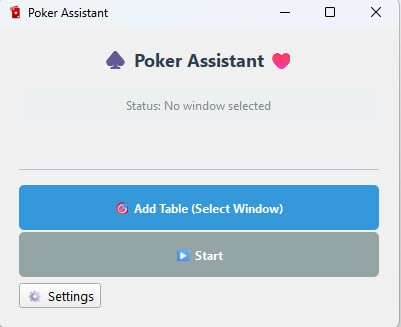
\includegraphics[width=0.6\textwidth]{images/app.jpg}
    \caption{Главное окно приложения}
    \label{fig:ui_hud}
\end{figure}

На рисунке~\ref{fig:ui_config} представлен пример конфигурационного интерфейса системы.

\begin{figure}[H]
    \centering
    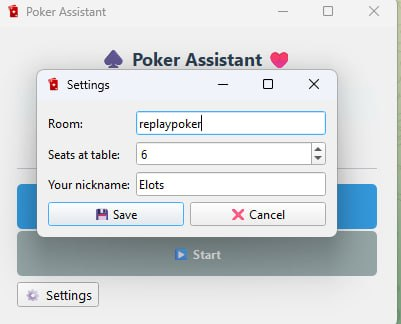
\includegraphics[width=0.8\textwidth]{images/config.jpg}
    \caption{Конфигурационный интерфейс системы}
    \label{fig:ui_config}
\end{figure}

На рисунке~\ref{fig:ui_advice} представлен оверлейный интерфейс с рекомендацией по действию.

\begin{figure}[H]
    \centering
    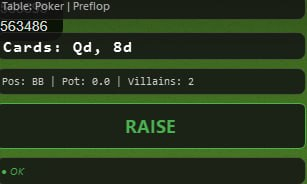
\includegraphics[width=0.6\textwidth]{images/advice.jpg}
    \caption{Оверлейный интерфейс с рекомендацией RAISE}
    \label{fig:ui_advice}
\end{figure}

\textbf{Пояснение к снимкам:}
\begin{itemize}
    \item все снимки сделаны с реальным покер-клиентом ReplayPoker;
    \item оверлейное окно не перекрывает карты игрока и кнопки действий;
    \item текст рекомендации выделен цветом и крупным шрифтом для быстрого восприятия;
    \item статусная строка внизу показывает техническую информацию (не мешает игре).
\end{itemize}

Таким образом, разработанный интерфейс обеспечивает баланс между информативностью и минимализмом, что позволяет игроку быстро получать необходимые рекомендации без отвлечения от основного игрового процесса.
